%\usepackage[top=0.5cm,bottom=0.5cm,left=0.5cm,right=0.5cm]{geometry}
%\usepackage[a5paper,top=0cm,bottom=0cm,left=0cm,right=0cm]{geometry}
\usepackage{listings}
\usepackage{color} %red, green, blue, yellow, cyan, magenta, black, white
\definecolor{mygreen}{RGB}{28,172,0} % color values Red, Green, Blue
\definecolor{mylilas}{RGB}{170,55,241}
\usepackage[swedish,english]{babel}
\usepackage[utf8]{inputenc}
\usepackage{amsmath}
\usepackage{graphicx}
\usepackage{float}
\usepackage{subfiles}
\usepackage{hyperref}
\usepackage{caption}
\usepackage{lipsum}
\usepackage{listings}
\usepackage{listingsutf8}
\usepackage{xcolor}
\usepackage{textcomp}
\usepackage{units}
\usepackage{bbm}
\usepackage{url}
\usepackage[english]{isodate}
\usepackage{gensymb}
\usepackage{amssymb}
\usepackage{amsthm}
\usepackage{fullpage}
\usepackage{tikz}
\usepackage{pgfplots} 
\usepackage{pgfgantt}
\usepackage{pdflscape}
\pgfplotsset{compat=newest} 
\pgfplotsset{plot coordinates/math parser=false}
\usepackage{todonotes}
\usepackage{siunitx}
\usepackage{geometry}
\usepackage[utf8]{inputenc}
\usepackage[T1]{fontenc}
\usepackage[english,swedish]{babel}
\usepackage{amsmath}
\usepackage{ae} 
\usepackage{units}
\usepackage[version=4]{mhchem}
\usepackage{icomma}
\usepackage{color}
\usepackage{graphicx}
\usepackage{bbm}
\usepackage{textcomp}
\usepackage{hyperref}
\usepackage{verbatim}
\usepackage{wrapfig}
%\usepackage{natbib}
\usepackage{multirow}
\usepackage{subfig}
\usepackage[titletoc]{appendix}
\usepackage{float}
\usepackage{parskip}
\newcommand{\HRule}{\rule{\linewidth}{0.5mm}}
\usepackage{chemfig} %https://en.wikibooks.org/wiki/LaTeX/Chemical_Graphics
\usepackage[backend=biber,style=ieee]{biblatex}
%https://www.tablesgenerator.com/
%https://www.codecogs.com/latex/eqneditor.php
% om man behöver få in vissa saker som SO4 men vill ha det underline så kan man gå in i "mathmode" genom att ha $"mattegrej$ typ $_{4}$ för att göra fyran nedsänkt % här ligger även bra hemsidor som man kan använda
\addbibresource{references.bib}
%\bibliography{references}
\begin{document}

\begin{titlepage}
\begin{centering}

{\huge\bfseries Vanadinutvinning från LD slagg som använts som syrebärare i förbränningsprocesser. \par}
\vspace{1cm}
{\scshape\Large \textbf{}\par}
{\scshape\Large \par}
{\Large\itshape Victor Hernvall, Frida Tropp,  \\ Timmie Dzafo Paulsson, Marcus Mellqvist \\ Stefan Ewaldsson, och Marcus Thim.\par}
{\large \today\par}

{   \par}
{   \par}
{    \par}


\begin{figure}[!ht]
\centering

\includegraphics[scale=0.3]{chalmers.png}
\label{fig:chalmers}

\end{figure}
\centering{\textbf{CHALMERS TEKNISKA HÖGSKOLA} \par}


\end{centering}
\end{titlepage}

\newpage 
\thispagestyle{empty}
\pagenumbering{roman}
\setcounter{page}{3}
\hspace{0pt}
\begin{centering}


\vfill
\Large Stort tack till Fredrik Hildor, Duygu Yilmaz, och Henrick Leion.
\vfill
\end{centering}
\hspace{0pt}
\begin{centering}
\topskip15pt
\end{centering}
\newpage
\thispagestyle{empty}
\begin{abstract}

Abstract

\end{abstract}

\newpage
\thispagestyle{empty}
\tableofcontents
\thispagestyle{empty}
\newpage
\pagenumbering{arabic}

%bakgrund 
% Börja med stålindustrin, masugn etc
% Teori LD-slagg
% Vanadin

% Förbränning
% Fluidiserad bädd
% Syrebärare  
% Biomassa

\section{Bakgrund}
%Stefan: https://www.accessscience.com/content/steel-manufacture/653800


%%Vid framställning av stål bildas diverse restprodukter som exempelvis gasreningsstoft, gasreningsslam och just slagg. Gasreningsstoft är de små partiklar som följer med de gaser som bildas i ståltillverkningens varma processer. Dessa avskiljs i hög utsträckning tillsammans med rökgaser i diverse filtreringsanordningar. Stoften kategoriseras som torra eller våta och efter rening  bildar de gasreningsstoft respektive gasreningsslam. [Jernkontoret - Gasreningsstoft och -slam blir nya råvaror][Jernkontoret handbok] 

%Stålslagg förekommer i en rad olika typer som t.ex. ljusbågsugnsslagg och LD-slagg\cite{Pehlke2014a}.
%Slaggen kategoriseras utifrån vilken typ av ugn som använts vid framställning av råjärnet. Ljusbågsugnsslagg är restprodukt av skrotbaserad ståltillverkning medan LD-slagg är restprodukt i malmbaserad ståltillverkning\cite{Pehlke2014a}. Slagg kan brukas i diverse tillämpningar som exempelvis konstruktionsmaterial eller asfalt; detta för att minska uttaget av jungfruliga resurser. Dessutom använder Stålverken begagnat material som skrot för tillverkning av nya produkter; detta för att nyttja resurserna till sitt yttersta. [https://www.jernkontoret.se/sv/stalindustrin/tillverkning-anvandning-atervinning/restprodukter/slagg/][https://www.jernkontoret.se/sv/stalindustrin/tillverkning-anvandning-atervinning/atervinning-av-jarn-och-stal/] 

%Svenskt ståls branschorganisation Jernkontoret hävdar trots detta att 20\% av avfallet, där spår av vanadin kan hittas, hamnar på deponi hos antingen kommunal deponeringsplats eller en extern aktör\cite{PontusWestrin}. Det tål också att nämnas att det finns tillgängligt flera ton av gammalt deponerat slagg till förfogande som syrebärare följt av lakmaterial. %Notera att man här inte vet vad varken en syrebärare eller ett lakmaterial är. Kanske ta bort meningen alternativt flytta ner den?

%[https://www.jernkontoret.se/sv/stalindustrin/tillverkning-anvandning-atervinning/restprodukter/]
%Båda dessa citerade 04-02-2019 

%\subsection{Som syrebärare i förbränningsprocesser}
%Det har visat sig att LD-slagg har potential som en billig syrebärare i kemcyklisk förbränning (CLC), där två stycken fluidiserande bäddreaktorer nyttjas för att separera CO$_2$ vid förbränning \cite{Xu2017}. Syrebäraren, som i detta fallet är LD-slagg, oxideras i ena reaktorn genom tillförsel av syre. Denna förflyttas sedan till den andra reaktorn där bränslet reducerar LD-slagget, för tillbakaförsel till första reaktorn.  %Har freestylat detta. Glöm inte att jämföra med källa för att se så det stämmer!
 
%Syrebärare kan även nyttjas i Oxygen Carrier Aided Combustion (OCAC), d.v.s. förbränning i en fluidiserad bädd där bäddmaterialet består av just en syrebärande metall.
%Syftet är att transportera syre till bränslet i understökiometriska områden för att på så vis öka pannans effektivitet\cite{Zevenhoven2018}.
 
 %Förbränning av biomassa är något som förknippas med CO$_2$ neutrala utsläpp och även i vissa fall negativa CO$_2$ utsläpp i de fall koldioxidlagring nyttjas som exempelvis en kemcyklisk förbränning\cite{Zevenhoven2018}.

%Vid analys av LD-slagg som nyttjats som bäddmaterial i Chalmers 12 MW cirkulerad fluidiserad bädd-förbrännare hittades ett skal av vanadin och fosfor kring partiklarnas yttre hölje med SEM-EDX-teknik. Det finns skäl att testa om detta skulle kunna underlätta lakning av båda dessa komponenter.

\subsection{Svenskt stål}

Stålindustrin har utvecklats rigoröst sedan de rudimentära stenugnarna som användes på medeltiden för att konvertera järnmalm till stål. Numera finns ett stort urval av processer som kan tillämpas baserat på vilken typ av malm som används, vilka förutsättningar som finns på plats och vilken slutprodukt som önskas \cite{Pehlke2014a}.

Stålprocessen börjar med att järnmalm grävs upp ur jordskorpan. Malmen, som består av olika former av järnoxid, anrikas i flera steg. I slutet av denna process fås järnpellets med homogen storlek och sammansättning som sedan kan användas vid tillverkning av råjärn i en masugn. Järnpelletsen innehåller ca 65\% järn \cite{RobertVikman}.

Masugnen är det första stora steget på vägen till färdigt stål. Processen är noggrannt styrd och kontrollerad, men är i grunden förbluffande lik de system som användes redan på medeltiden. Järnpellets, koks och slaggbildare skiktas i lager i masugnen som eldas nerifrån med en forcerad luftström som ger en mycket hög förbränningstemperatur. När masugnens olika lager sjunker neråt matas den uppifrån med nytt material. I botten av ugnen samlas det smälta järnet och kan tappas av. Det avtappade järnet kallas råjärn och innehåller ca 4\% kol. Rent kemiskt reduceras järnmalmen med koks som reduktionsmedel enligt reaktion \eqref{eq:järnoxid} nedan.

\begin{equation}
    C+FeO \rightarrow CO + Fe(l)
    \label{eq:järnoxid}
\end{equation}

Särskilt intressant för denna studie är syrgasprocessen eller LD-processen, Linz Donawitz-processen, som uppfanns i Österrike på tidigt 1950-tal \cite{Jernkontoret2000del1}.
Processens namn kommer från de två Österrikiska städerna som först tillämpade processen kommersiellt. Denna process är ett av reningsstegen som följer på masugnen för att producera smidbart stål som i slutändan har en kolhalt på 0,04-0,8\% \cite{Jernkontoret2000del2}.
Råjärnet behöver gå igenom en oxidationsprocess för att oxidera ut det oönskade kolet enligt reaktion \eqref{eq:kolox} nedan.

\begin{equation}
    C +\frac{1}{2} O_{2}(g) \rightarrow CO(g)
    \label{eq:kolox}
\end{equation}

I LD-processen blåses syrgas ner i järnsmältan och åstadkommer förutom värmetillförsel den önskade oxideringen enligt \eqref{eq:kolox}. En av fördelarna med denna metod är den effektiva omrörningen av smältan och slagget som finns däri.

Slagget som nämns ovan är vad man kallar de komponenter som inte kommer ingå i det färdiga stålet och som man önskar avskilja. Under LD-processen och många andra metoder spelar dock slagget en avgörande roll  \cite{Slagg-Jernkontoret}. 
Slagget som bildas flyter ovanpå smältans yta till följd av densitetsskillnader. På ytan fyller slagget två viktiga funktioner, det fungerar som en värmesköld för smältan och är samtidigt en barriär mot luften som inte ska komma åt och oxidera järnsmältan. Utöver den skyddande rollen kan slagg binda in olika föroreningar som inte är önskvärda i stålet. För att åstadkomma detta kan olika slaggbildare tillsättassom är anpassade för att binda in diverse föroreningar beroende på vilka råmaterial som används. Främst används kalksten för detta \cite{RobertVikman}.

\subsection{LD-slagg}
LD-slagg är det som bildas vid en så kallad LD-konvertering som är en del av framställningen av stål från järnmalm. Denna restprodukt innehåller fortfarande en hel del användbara ämnen se, Tabell \ref{tab:LDslagg},  som till exempel fosfor och vanadin. Svensk järnmalm innehåller sällsynt stora mängder vanadin vilket medför att även LD-slagget har kvar stora mängder av det. År 2015 medförde stålindustrin att 309 362 ton av LD-slagg bildades som står för 16\% av alla restprodukter från stålindustrin \cite{Jernkontoretrest}. Där den överväldigande majoriteten av LD-slaggen läggs på deponi.

\begin{table}[H]
\caption{Sammansättning, i vikt\% , av obehandlad LD-slagg som från Sverige och gentemot från Nordamerika \cite{Proctor2000}. }
\begin{tabular}{|l|l|l|l|l|l|l|l|l|l|l|}
\hline
Provbehandling                                                                 & Fe    & Ca    & Mg   & Mn   & Al   & V    & K    & P    & Si   & S    \\ \hline
\begin{tabular}[c]{@{}l@{}}Svenskt\\ LD-slagg \\ obhandlat\end{tabular}        & 17.07 & 31.73 & 5.88 & 2.64 & 0.76 & 1.51 & 0.04 & 0.25 & 5.61 & 0.1   \\ \hline
\begin{tabular}[c]{@{}l@{}}Nordamerikanskt\\ LD-Slagg\\ obhandlat\end{tabular} & 28.55 & 43.4  & 8.57 & 5.1  & 3.69 & 0.15 & N/A  & 0.49 & 9.24 & 0.17 \\ \hline
\end{tabular}
\label{tab:LDslagg}
\end{table}

\subsection{Förbränningstekniker}
%Nyckelord: fast material, fluidisering, effektivitet, sand, agglomeration, negative emissions

Effektivare förbränningsprocesser är nödvändigt för att dels tackla de klimatproblem som kan relateras till utsläpp av växthusgaser, men också de ekonomiska aspekter som kan relateras till drift av anläggningar.

Detta har öppnat upp för diverse förbränningstekniker där syrebärare spelat en central roll i förbättringsarbetet. Syrebäraren, som kan vara metalloxid, har i uppgift att minska lufttillförsel i processen vilket resulterar i mindre NO$_X$-utsläpp och billigare drift \cite{doi:10.1021/acs.energyfuels.7b00197}.

\subsubsection{Chemical-looping combustion}
Chemical-looping combustion, CLC, på svenska kemcyklisk förbränning, är en teknik vars syfte är att lagra CO$_2$ i en förbränningsprocess. Två stycken fluidiserade bäddreaktorer; en för bränsletillförsel och en annan för lufttillförsel, kan nyttjas för att separera CO$_2$ och H$_2$O i förbränningsprocessen.

För att transportera syre från luft- till bränslereaktorn nyttjas en syrebärare. Syrebäraren cirkuleras fram och tillbaka mellan reaktorerna för att växelvis oxideras och reduceras i processen. Förloppet illustreras i Figur \ref{fig:CLC} nedan.

\begin{figure}[H]
    \centering
    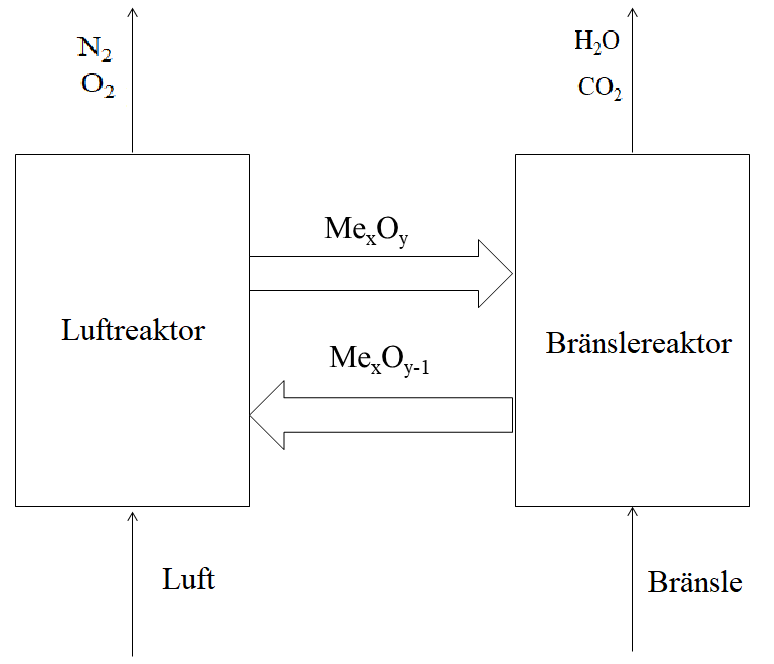
\includegraphics[scale=0.4]{CLC.png}
    \caption{Konceptuell skiss över en CLC-process}
    \label{fig:CLC}
\end{figure}

Oxidationen och reduktionen av syrebäraren kan beskrivas i ett reduktionssteg \eqref{eq:reduktion} följt av ett oxidationssteg \eqref{eq:oxidation} enligt reaktionschemat nedan

\begin{equation}
C_nH_2m+(2n+m)Me_xO_y \rightleftharpoons  CO_2+mH_2O+(2n+m)Me_xO_{y-1}
   \label{eq:reduktion}
\end{equation}
\begin{equation}
    O_2 + 2Me_xO_{y-1} \rightleftharpoons  2Me_xO_y
    \label{eq:oxidation}
\end{equation}

där CnH$_2$m är ett godtyckligt bränsle och Me är den metall som agerar syrebärare \cite{OresHenrik}.

\subsubsection{Oxygen Carrier Aided Combustion}
I konventionella fluidiserande bäddpannor så används sand som bäddmaterial. Tanken med Oxygen Carrier Aided Combustion (OCAC) är att man istället för sand använder ett syrebärande material, som ofta är en metalloxid \cite{doi:10.1021/acs.energyfuels.7b00197}. Detta gör att bäddmaterialet även fördelar syre jämnt i pannan och inte bara värme.

\subsubsection{Förbränning av biomassa}
Det som skiljer förbränning av biomassa från många andra bränslen är att biomassa har större variation på sin sammansättning \cite{Ashcomp}. Biomassa innehåller framförallt alkaliska ämnen som i en fluidiserad bäddpanna kan reagera med bäddmaterialet och då resultera i att bäddmaterialet agglomererar och då förhindrar fluidisering \cite{Alkali}-\cite{glas}. Detta innebär att pannan måste stannas för rengöring och utbyte av bäddmaterial måste ske.

Biomassaförbränning i CLC förknippas även med negativa nettoutsläpp av CO$_2$. Efter förbränningen i CLC:n förvaras CO$_2$ i hålrum under marken för att permanent tas bort ur atmosfärens kolkretslopp, vilket i slutändan leder till ett negativt nettoutsläpp av CO$_2$ \cite{Bui2018}.
%-CLC biomassa negativ emission
% Beor på att man förvarar CO2 i bergrund
%

\subsubsection{Syrebärande bäddmaterial}
%Här pratar vi om olika malmer
%Dit kommer vi till LD-slagg
Det faktum att bäddmaterial agglomererar vid biomassaförbränning resulterar i att bäddmaterialet behöver bytas ut med jämna mellanrum. Därför är billiga och effektiva syrebärare av intresse.  
Den skall inte bara uppvisa hög reaktivitet med avseende på oxidation och reduktion, utan även vara billig och ha en så låg miljöbelastning som möjligt. 

Malmer med höga halter övergångsmetaller som antingen mangan eller järn har visat sig fungera väl som syrebärare.
En järnbaserad mineral som i huvudsak består av FeTiO$_3$, ilmenit,  har varit av intresse för en omfattande mängd studier, och även andra ämnen innehållande järn och mangan är av intresse \cite{OresHenrik},\cite{Xu2017}.

%Deponerat LD-slagg ...för att möta behovet av en billig syrebärare.
Behovet av billiga syrebärare har lett till att LD-slagg setts som en möjlig kandidat på grund av dess järnhalt. Svenskt deponerat LD-slagg har därför testats i Chalmerspannan som syrebärande bäddmaterial för att möta behovet av en billig syrebärare \cite{chalmerspanna}.

%Ilmenite, hematite

\subsection{Lakning LD-slagg}

Opublicerad forskning av en syrebärarforskningsgrupp på Chalmers har visat att vanadin förflyttar sig mot ytan av LD-slagg partiklarna då de använts som syrebärare. Att koncentrationen på ytan ökar medför att det potentiellt skulle kunna underlätta utvinningen av ämnet. Det har även visat sig att fosfor från bränslet annsamlas på partikelytan, vilket medför att det potentiellt finns möjligheter att ta tillvara på fosfor i samband med vanadinutviningen. En möjlig separationsmetod skulle kunna vara lakning.

\subsubsection{Lakning}

Lakning bygger på att lösa upp en löslig del av ett material och på så vis skilja den från den olösliga delen. Det finns två huvudgrupper av lakning, där lösningsmedlet antingen rinner igenom lakgodset eller där lakgodset tillsätts i lösningsmedlet. Lösningsmedlet kommer antingen att lösa ämnena direkt eller reagera med dem så att produkten kan lösas i lösningsmedlet. Lakning gynnas av en ökad kontaktyta och en liten partikelstorlek är därmed gynnsamt \cite{lakning}. 




\subsubsection{Vanadin och fosfor}

Vanadin, grundämne nummer 23, är en övergångsmetall i det periodiska systemets femte grupp. Vanadin hittas i en handfull olika tillämpningsområden som exempelvis katalysator i en rad olika tillverkningsprocesser \cite{Pecoraro2014}.
Metallen har oxidationstillstånd, +2,+3,+4 och +5 \cite{Baroch2013}. Vilket har gjort att metallen varit av särskilt intresse i flödesbatterier och därför föremål för studier ända sedan förra århundradet \cite{Skyllas-Kazacos1987}.
Fördelen med de många oxidationstillstånden är att elektrolyterna i batteriets halvceller kan bestå av samma metall vilket är fördelaktigt med avseende på kontaminering av membran, elektrod och elektrolyter 
\cite{Lopez-Vizcaino2017}. Vanadin nyttjas dock mest som ett additiv i ståltillverkning vars syfte är att stärka stålet, avseende både hårdhet och hållfasthet \cite{Baroch2013}. Bland annat används en stor del av vanadinet som en legering för stål inom olika användningsområden, exempelvis balkar, armeringar och stålrör \cite{Pecoraro2014}. Vanligtvis så behöver vanadin tillsättas till stålet vid tillverkningen, men de höga mängderna naturligt förekommande vanadin i svensk järnmalm räcker för att producera högkvalitativt stål utan vidare tillsaster. 

Fosfor, grundämne nummer 15, är en icke-metall i periodiska systemets tredje grupp. Den främsta användningen för fosfor är inom jordbruket i form av konstgödsel. Utvinning av fosfor sker främst ur mineraler, då i form av fosfater. Eftersom fosfor är en begränsad resurs finns ett stort värde i att ta hand om alla materialströmmar som kan innehålla användbara kvantiteter av ämnet. LD-slagget har vid analys uppvisat en (specificera) halt fosfor som eventuellt skulle kunna tas till vara på i samband med lakningsprocessen avseende vanadin \cite{VanWazer2018}.

%I dagens samhälle ökar behovet av förnybar energi i form av exempelvis solkraft för att ersätta fossila alternativ. Detta yttrade sig tydligt i Sverige 2018 då intresset för solkraft ökade som ett svar på regeringens beslut om utökat investeringkostnadsstöd från 20 till 30 procent i solcellsinstallationer från och med den första januari 2018\cite{SverigesEnergimybn2009}.

%Problemet som kvarstår är dock att förnyelsebara energikällor i allmänhet och solceller i synnerhet inte producerar elektricitet i paritet med efterfrågan; förnyelsebara elnät är överlag känsliga mot de fluktuationer som uppstår i elnätet. Lösningen på ett av dagens energiproblem skulle alltså kunna lösas genom att lagra energin med flödesbatterier av vanadintyp\cite{Lopez-Vizcaino2017}.



\section{Samhälleliga och etiska aspekter}
Det finns en  väldigt stor industri som tillämpar LD-processen för att tillverkar stål. Till följd av detta finns även en väldigt stor sidoström innehållande stålslagg, kallat LD-slagg. Detta slagg läggs i nuläget på deponi, vilket skulle kunna vara en negativ samhällelig aspekt om det hanteras illa. En felaktigt hanterad deponi skulle kunna leda till läckage av tungmeteller eller fosfor till närliggande vattendrag. Det skulle även kunna vara så att deponin läggs på ett ställe där den blir skrymmande eller stör utsikten. 

% En mer etisk aspekt av deponin vore i fallet att exempelvis tungmetaller och fosfor läcker ut i närliggande vattendrag eller jordmån.

Att använda slaggen som syrebärare är ett effektivt sätt att utnyttja restprodukter från en annan process, som är lättillgänglig och finns i stora kvantiteter. Går det dessutom att laka vanadin och kanske även fosfor bidrar det till en mer hållbar och cyklisk process. Det medför även ett minskat behov av att bryta malm med avsikt att utvinna fosfor. 





% Genom att använda LD-slagg som syrebärare i förbränningsprocesser och vidare laka den brända slaggen för utvinning av vanadin ger en hållbar och cyklisk process som utnyttjar restprodukter från en annan process som är lättillgänglig och finns i stora kvantiteter.

\section{Syfte}
%Syftet med arbetet är således att testa om lakning av LD-slagg som befunnit sig i en fluidiserad bädd är en tillfredsställande metod för utvinning. Detta skulle kunna stänga materialkretslopp med avseende på inte bara vanadin utan eventuellt också fosfor och LD-slaggets livstid skulle kunna förlängas gentemot dagens spann. När lakning har utförts kommer det också analyseras i vilka typer av lakningsbara faser vanadinet finns i och hur dessa skulle kunna tänkas efterbehandlas. 

Detta arbetes syfte är att ta reda på i vilken grad det går att laka ur vanadin ur LD-slagg, som har används som bäddmaterial i Chalmerspannan, med hjälp av svavelsyra. Med detta kan det vara möjligt att öka LD-slaggets användningsområden och sluta materialkretsar som i nu läget deponeras på hög. 
\section{Problem}
Den huvudsakliga uppgiften består i att jämföra möjligheterna att utvinna vanadin ur LD-slag som har genomgått olika behandlingar innan lakning.

%Deluppgift ett kommer bestå i att utföra en rad experiment som undersöker under vilka förhållanden och i vilket medium, d.v.s syra, som lakningen är mest gynnsam.

     

Deluppgift ett kommer att bestå av att utföra experiment på vilken koncentration av svavelsyransyran som är mest gynnsam för lakning. 

Deluppgift två kommer att vara att ta reda på vilken temperatur som är mest gynnsam för lakningen. 

%ändra detta då vi bara kommer titta på syra i nuläget

Deluppgift tre kommer innefattar att identifiera vilken förhållande mellan syra och LD-slagget som är den mest optimala. 

Deluppgift fyra innefattar att analysera de olika filtratet från lakningen med hjälp av AAS. Samt att analysera, förutsatt att det inte är helt upplöst av syran, lakgodset med hjälp av XRD. % Hade velat flytta "lakgodset" så att det står mellan analysera och ,

I mån av tid kan det även testas huruvida det är möjligt och i vilken mängd fosfor kan urlakas från LD-slagget. 
tid kan det även testas huruvida det är möjligt och i vilken mängd fosfor kan urlakas från LD-slagget. 

%Utöver de test som kommer göras för att analysera mängden utvunnen vanadin kommer det även testas vilken halt fosfor som erhålls i samma prov.

\section{Metod}

 

Valet av metod grundar sig i tidigare uppställningar för liknande laborationer, samt en laborations uppställning som visas av handledaren Duygu Yilmaz\cite{Aarabi-Karasgani2010}. Experimentuppställningen består av en trehalsad rundbottenskolonn som befinner sig i ett vattenbad på en värmeplatta med magnetomrörning. Till de tre halsarna så är en av halsarna försedd med en kork, en med en termometer, och slutligen en med kondensor se i Figur \ref{fig:labupp}, samt Figur \ref{fig:labbild}. Temperaturen, ration mellan vätska och fast ämne, samt koncentration på syran väljs beroende på vilken kedja av experiment som utförs, se tabell \ref{tab:metodtab}. Lakningen sker genom att 1 gram av LD-slagget tillsätts till H$_{2}$SO$_{4}$, som är förvärmt till rätt temperatur för det experimentet. Omrörningen har bestämts till 360 rpm. Provet lakas i 2 timmar och provtagningen sker i intervallerna 30 minuter, 60 minuter, 120 minuter. Vid provtagning plockas 1 ml upp av provet. Efter att lakningen är gjord så filteras provet med en Büchner tratt med ett glasfilter och ett pappersfilter. Provet är nu efter detta redo för att analyseras med en AAS. 
\begin{figure}[H]
    \centering
    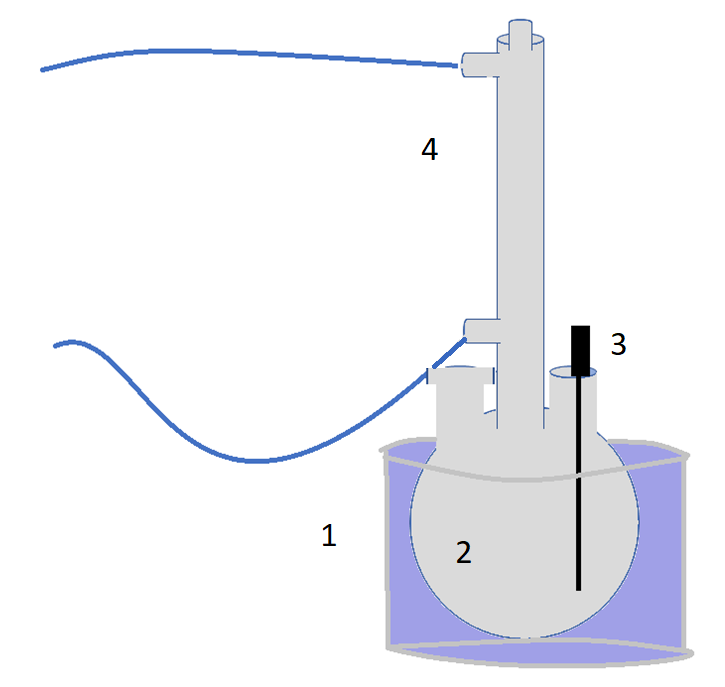
\includegraphics[scale=0.4]{labbupp.png}
    \caption{Laborations uppställningen i nuläget. 1. Vattenbad som värms upp med en värmeplatta. 2. Trehalsad rundbottenskolonn. 3. Termometer som är kopplad till värmeplatten. 4. Kondensor.    }
    \label{fig:labupp}
\end{figure}

\begin{table}[H]
\caption{Premilinär test uppställning.}
\begin{tabular}{|l|c|c|c|}
\hline
\textbf{\begin{tabular}[c]{@{}l@{}}Parametrar\end{tabular}}              & \multicolumn{1}{l|}{\textbf{\begin{tabular}[c]{@{}l@{}}H$_{2}$SO$_{4}$ \\ koncentration [M]\end{tabular}}} & \multicolumn{1}{l|}{\textbf{\begin{tabular}[c]{@{}l@{}}Ratio mellan vätska \\ fast och  [ml/g]\end{tabular}}} & \multicolumn{1}{l|}{\textbf{\begin{tabular}[c]{@{}l@{}}Laknings\\ Temperatur  [$\degree$C]\end{tabular}}} \\ \hline
\textbf{\begin{tabular}[c]{@{}l@{}}H$_{2}$SO$_{4}$ \\ koncentration [M]\end{tabular}}    & 3,4,5                                                                                                    & 25:1                                                                                                           & 70                                                                                                        \\ \hline
\textbf{\begin{tabular}[c]{@{}l@{}}Ratio mellan vätska\\ och fast [ml/g]\end{tabular}} & 3                                                                                                          & 25:1, 50:1, 100:1                                                                                            & 70                                                                                                        \\ \hline
\textbf{\begin{tabular}[c]{@{}l@{}}Laknings \\ Temperatur  [$\degree$C]\end{tabular}}    & 3                                                                                                          & 25:1                                                                                                           & 50, 60, 70, 80                                                                                               \\ \hline
\end{tabular}
\label{tab:metodtab}
\end{table}

 Ett flertal metoder kommer att användas för att analysera proverna. Atomabsorptionsspektroskopi, AAS, och röntgenkristallografi, XRD från engelska X-ray diffraction, och svepelektronmikroskopi, SEM. De olika metoderna används för olika delar av arbetet. AAS används för att undersöka om vanadin har lakats ur LD-slagget. XRD kommer att användas för att analysera kristallstrukturen av LD-slagget före och efter att det har rostats och vid olika intervaller under rostningen för att se sammansättningen av de olika ämnena i kristallen. Slutligen så kommer SEM användas för att se var i LD-slagget som de olika ämnena befinner sig i slaggpartiklarna. 

En litteraturstudie ska ske parallellt med laborationerna för att kunna ge möjlighet till djupare inlärning och förklaring av ämnet. Detta innebär användningsområden av vanadin, användadet av LD-slagg och dess deponering i nuläget. Även vilka fördelar och nackdelar processen har och vad det kan göra för samhällsnytta inför i framtiden. 
\section{Avgränsningar}

%Även om det är ett ämnes område som det i nuläget redan görs forskning på, inom olika applikationer och djupare förståelse, så finns det mycket potential i det här projektet. Men det med begränsade resurser, främst tid, så kommer vi behöva göra en mängd avgränsningar på vad som kommer att kollas på. 

%Liknande projekt som detta arbetas på i nuläget. Men de projekten rostar LD-slagget snarare än att använda det som en syrebärare i den fludiserade bädden av ett värmekraftverk. Då detta är en unik möjlighet så krävs det att avgränsningar sker tidigt för att kunna fokusera på ett spetsområde.  

Arbetets främsta begränsning kommer att vara tid. Detta medför att i mån av tid skulle avgränsningarna kunna utvidgas något. Till att börja med kommer arbetet att  begränsats till att bara undersöka lakning med svavelsyra. Dessutom kommer endast tre olika parametrar undersökas,temperatur, syrans koncentration, och förhållande mellan vätska och fast fas, trots att det finns många fler som påverkar. Försöken kommer utöver detta variera en parameter i taget medans de andra parametrarna hålls konstanta. I mån av tid kommer det att även undersökas huruvida fosfor urlakas ur LD-slagget.  

%Det här arbetet kommer inte heller ta hänsyn till ekonomiska och kemitekiska optimeringar. Det innebär optimering av storskaliga system eller hur det ska tillämpas på en uppskallad process. Detta görs i avseende av att det är inte projektet syfte, samt att det kommer att innebära en ännu större litteraturstuide än vad som är planerat.
\section{Tidsplan}
Tidsplanen som skall följas finns lättöverskådligt i Appendix \ref{appendix}, där Figur \ref{fig:Ganttliten} är ett Gantt-schema som veckovis ger en överblick över projektet och Figur \ref{fig:Ganttroterad} är ett mer utförligt Gantt-schema på dagbasis för projektet. Schemat är preliminärt och viss ändring kan ske, exempelvis kan laborationsarbetet pågå längre än planerat eller avslutas tidigare beroende på hur labbarbetet kommer gå.

\newpage
\printbibliography
\thispagestyle{empty}
\newpage
\appendix
\section{Appendix} \label{appendix}
\pagenumbering{roman}
\begin{figure}[H]
    \centering
    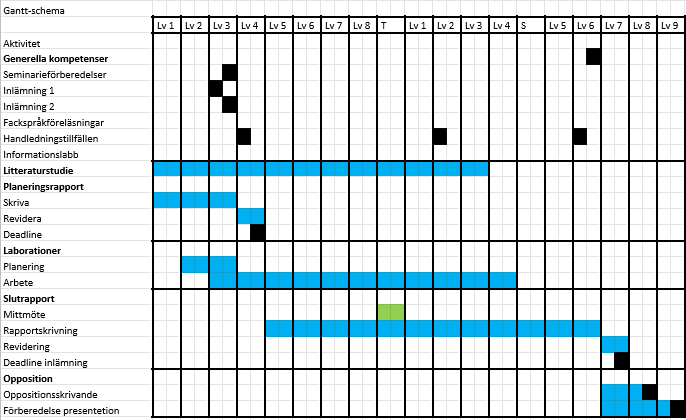
\includegraphics[scale=0.8]{Ganttliten.PNG}
    \caption{Gantt-schema över veckorna relaterat till projektbeskrivningen}
    \label{fig:Ganttliten}
\end{figure}

\newpage
\thispagestyle{empty}
\begin{figure}[H]
    \centering
    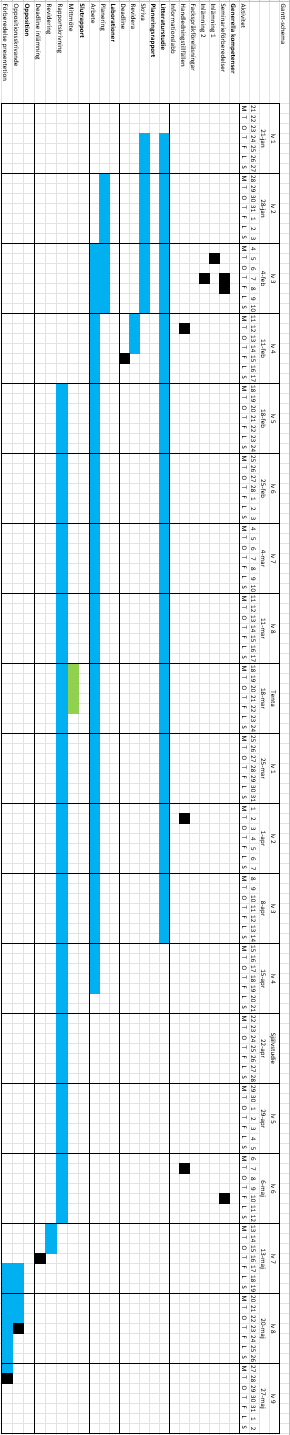
\includegraphics[scale=0.6]{Ganttroterad.PNG}
    \caption{Gantt-schema över hela projektet, dag för dag}
    \label{fig:Ganttroterad}
\end{figure}
\newpage
\thispagestyle{empty}
\begin{figure}[H]
    \centering
    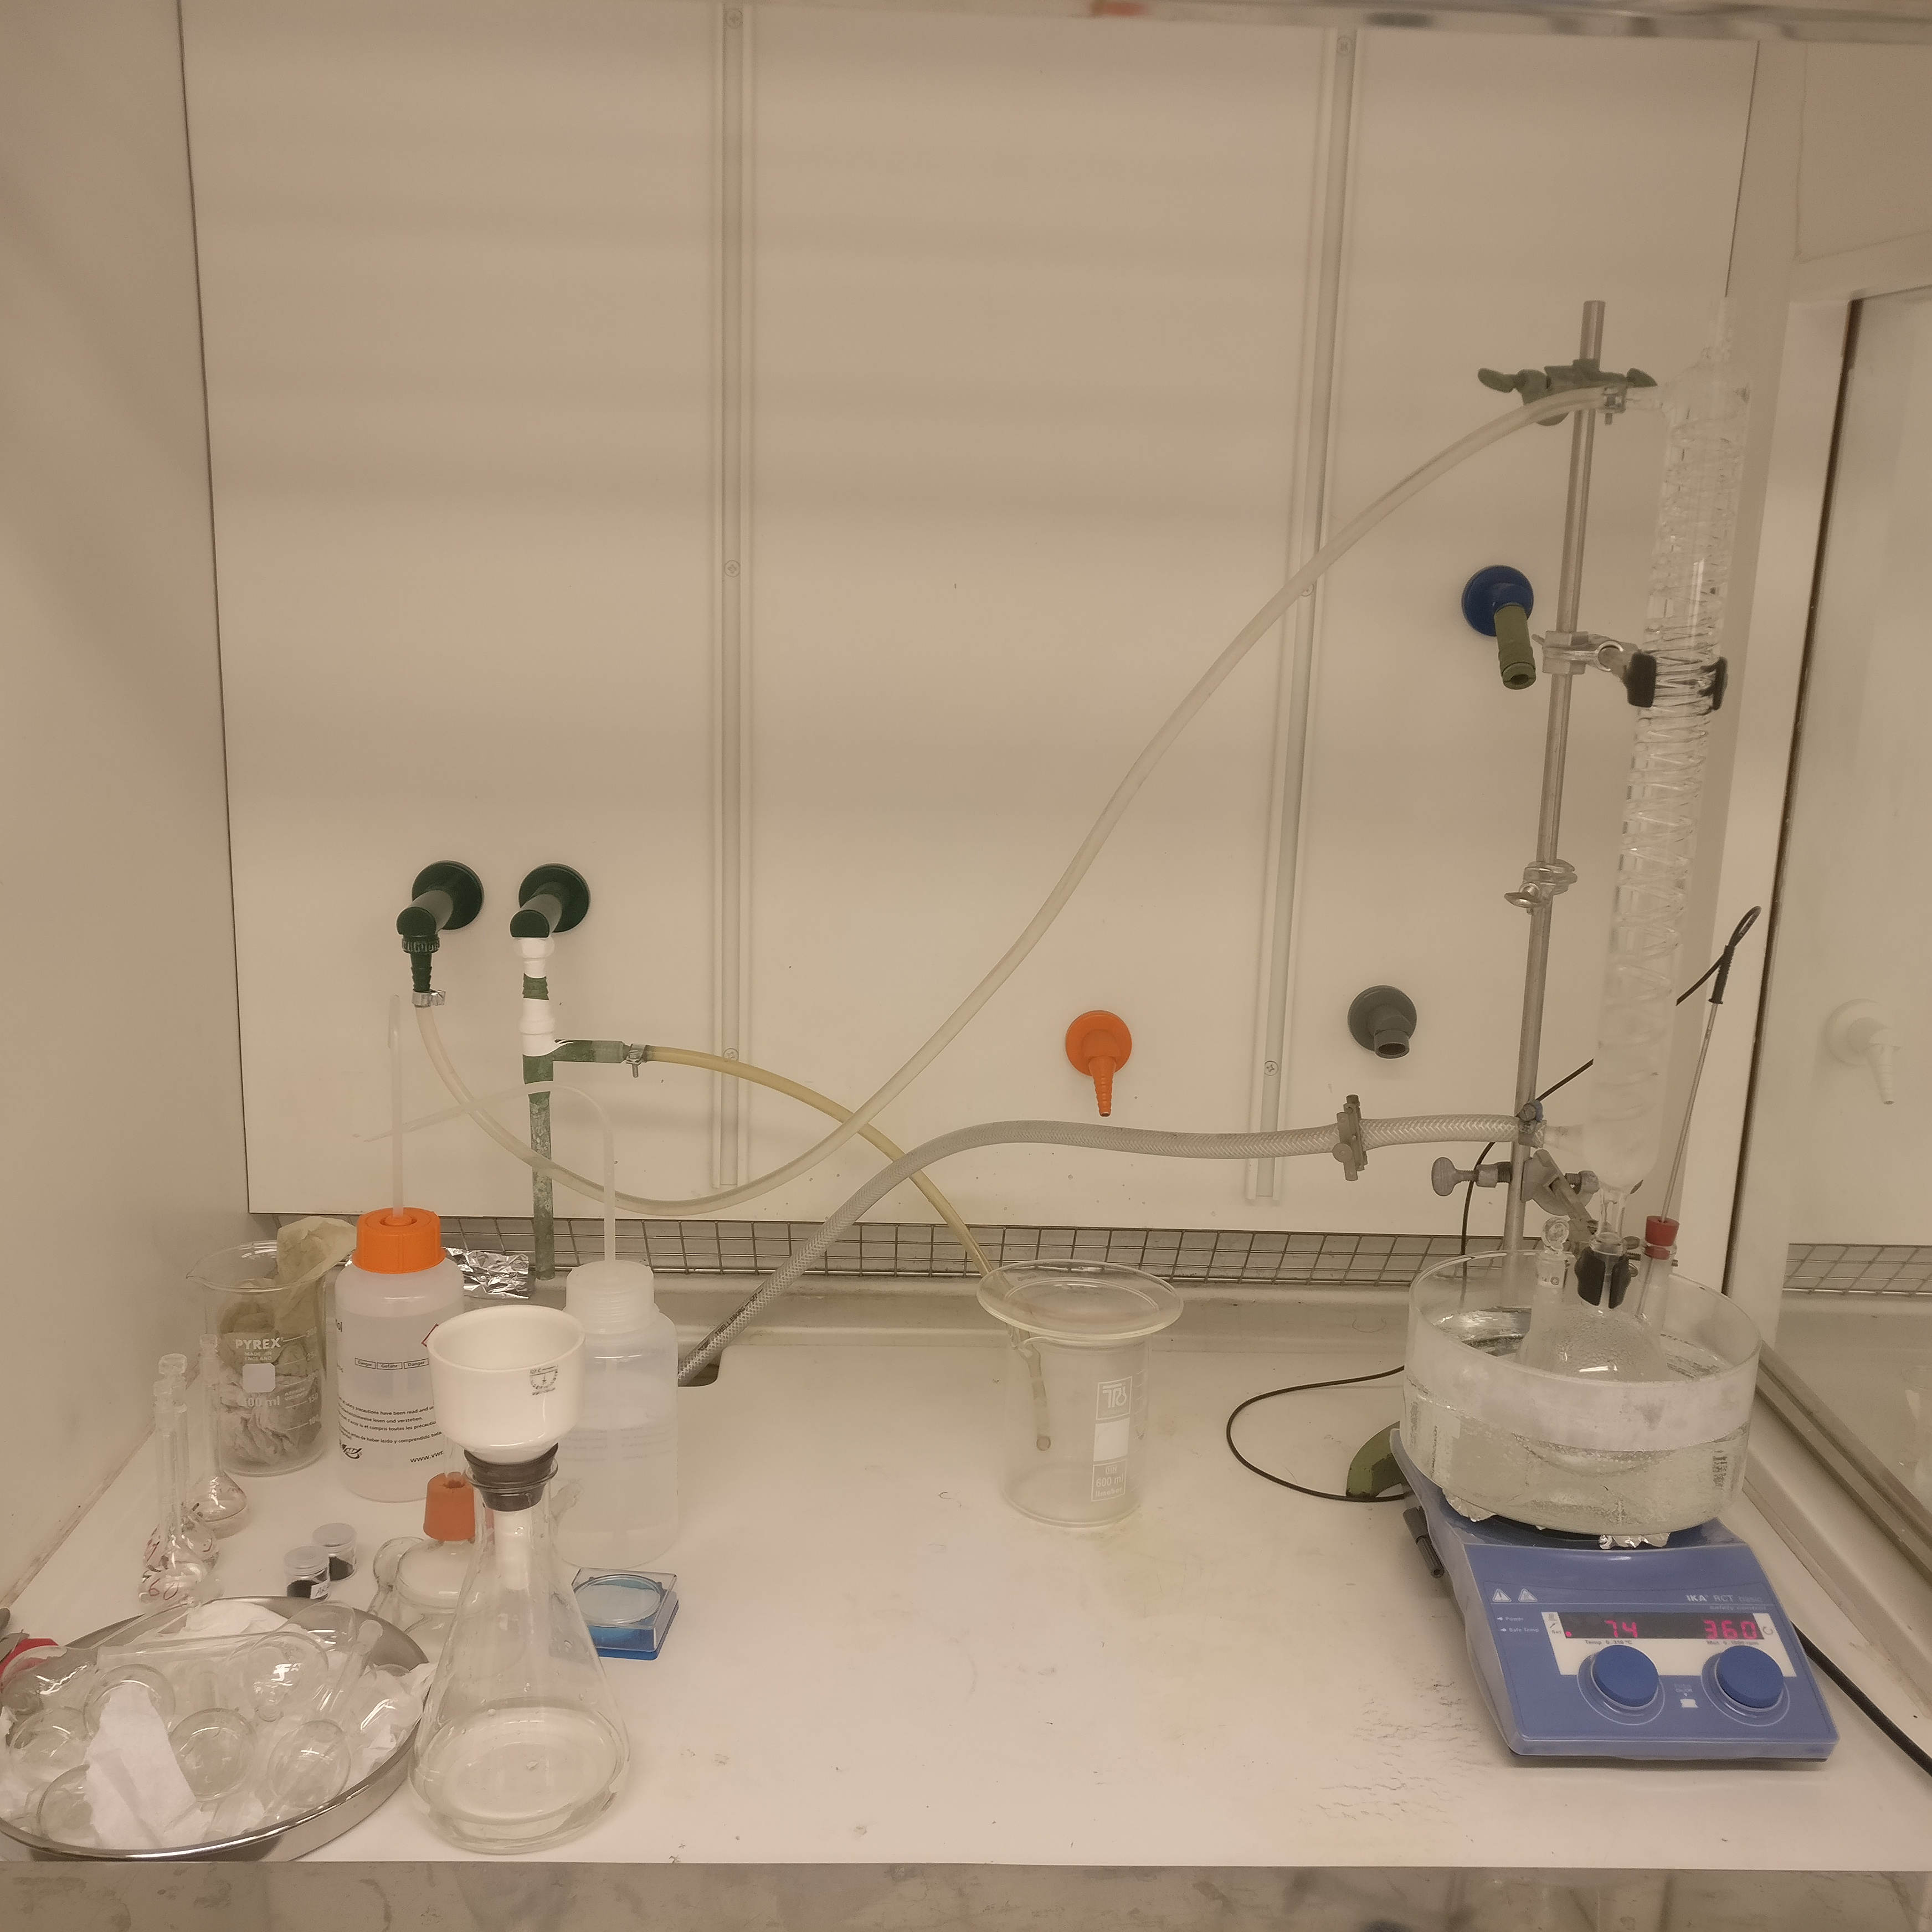
\includegraphics[scale=0.1]{labsetup.jpg}
    \caption{Laborations uppställningen i nuläget.}
    \label{fig:labbild}
\end{figure}

\end{document}

